\documentclass[11pt,a4paper]{article}

% ── Packages ───────────────────────────────────────────────────
\usepackage[utf8]{inputenc}
\usepackage[T1]{fontenc}
\usepackage{amsmath,amssymb,amsfonts}
\usepackage{bm}
\usepackage{graphicx}
\usepackage{booktabs}
\usepackage[margin=2.5cm]{geometry}
\usepackage[numbers]{natbib}
\usepackage{hyperref}
\usepackage{algorithm}
\usepackage{algorithmic}
\usepackage{xcolor}
\usepackage{float}

\hypersetup{
    colorlinks=true,
    linkcolor=blue,
    citecolor=blue,
    urlcolor=blue,
}

% ── Title ──────────────────────────────────────────────────────
\title{Bayesian Cross-Validation for Automatic Relevance Determination\\in Sparse RS-HDMR Surrogate Construction}
\author{Frederick Bennett\\
\textit{Department of Environment, Tourism, Science and Innovation}\\
\textit{Queensland Government, Brisbane, Australia}}

\date{May 2026}

\begin{document}
\maketitle

\begin{abstract}
Automatic Relevance Determination (ARD) is a sparse Bayesian learning algorithm widely used for feature selection in high-dimensional regression. When applied to Random Sampling--High Dimensional Model Representation (RS-HDMR) surrogate construction for sensitivity analysis, the ARD algorithm produces a path of candidate models with increasing numbers of active basis functions. Selecting the model with optimal predictive performance requires a criterion beyond ARD's internal convergence test. We present a retrospective $K$-fold cross-validation methodology using the Bayesian predictive log-likelihood as a scoring function. The score is derived from the full ARD predictive distribution and provides a principled, probabilistic criterion for model selection. We correct a subtle but consequential data-leakage issue---per-fold centering with full-dataset statistics---that produces systematically optimistic CV scores. The methodology is demonstrated on two benchmark case studies: the Ishigami function ($d=3$) and the Sobol--Levitan wing weight function ($d=10$). On the Ishigami function, the Bayesian CV score yields $R^2=0.999$ and recovers analytical first-order Sobol indices within $0.3\%$. The retrospective selection architecture matches the design of scikit-learn's Orthogonal Matching Pursuit CV and is implemented in the open-source ShapleyX package.  The implementation also provides a batch evidence-maximization ARD variant with Gamma hyper-priors, matching sklearn\textquotesingle s \texttt{ARDRegression} sparsity behaviour while retaining the Bayesian CV model selection infrastructure.
\end{abstract}

% ====================================================================
\section{Introduction}
% ====================================================================

Global sensitivity analysis quantifies how uncertainty in model inputs propagates to uncertainty in model outputs \citep{saltelli2008}. The Sobol variance decomposition \citep{sobol2001} and Shapley effects \citep{owen2014,song2016} are the dominant tools, but their estimation requires thousands to millions of model evaluations---prohibitively expensive for computationally intensive simulators.

Surrogate modelling addresses this by constructing a cheap-to-evaluate approximation of the original model. The Random Sampling--High Dimensional Model Representation (RS-HDMR) \citep{li2002,rabitz1999} builds an expansion in terms of shifted Legendre polynomials with coefficient sparsity enforced through regularised regression. The expansion order and degree are controlled by a parameter vector $\mathbf{p} = [p_1,\dots,p_m]$ specifying per-interaction-order polynomial degree caps. For $d$ inputs, this yields $N_{\text{feat}} = \sum_{k=1}^{m} \binom{d}{k} p_k^{\,k}$ candidate basis functions---ranging from tens (small $d$, low $p_k$) to hundreds of thousands (large $d$, high-degree interactions).

\textbf{The scalability problem.}  For a typical RS-HDMR problem with $d=20$ and $\mathbf{p}=[8,6,4]$, the design matrix $\mathbf{X}$ occupies $6.4$~GB at $n=10^4$ and the Gram matrix $\mathbf{X}^T\mathbf{X}$ occupies $51$~GB---exceeding the memory of commodity hardware.  The batch evidence-maximization ARD algorithm used by sklearn's \texttt{ARDRegression} \citep{mackay1992} requires the full $\mathbf{X}^T\mathbf{X}$ to iterate closed-form update rules for all $p$ weights simultaneously.  At $p > 10^4$ this becomes infeasible: the $p \times p$ Gram matrix alone demands tens of gigabytes, and each iteration performs $O(p^2)$ operations on it.

\textbf{Why a greedy algorithm is necessary---and why it needs help.}  The fast sequential SBL algorithm of \citet{tipping2003} solves the scalability problem by operating on only one feature at a time.  Instead of maintaining the full $\mathbf{X}^T\mathbf{X}$, it maintains $\mathbf{X}^T\mathbf{X}_{\text{active}}$---a $(p \times |\mathcal{A}|)$ matrix that grows incrementally with the active set.  For typical RS-HDMR surrogates where $|\mathcal{A}| \approx 50$--$200$, this reduces memory by three orders of magnitude.  However, the sequential algorithm's internal convergence criteria---no features added or deleted, and small changes in existing feature precisions---guarantee a stationary point of the marginal likelihood but provide no guarantee of optimal predictive performance.  Marginal features whose individual $q_i^2 - s_i > 0$ criterion narrowly passes the threshold accumulate slowly across iterations; the convergence point may contain dozens of features that contribute little to generalisation but inflate the model complexity.

\textbf{Our solution.} We couple the scalable sequential ARD algorithm with retrospective $K$-fold Bayesian cross-validation evaluated along the full iteration path.  The greedy algorithm explores the sparsity landscape one feature at a time on the full dataset, exploiting its $O(p \times |\mathcal{A}| \times n)$ memory footprint to handle $p > 10^4$ candidate features.  At each iteration the visited model state is scored via CV using the Bayesian predictive log-likelihood---a principled metric that accounts for both prediction accuracy and predictive uncertainty.  After convergence (or a fixed budget of iterations), the state with the highest CV score is retrospectively selected, discarding marginal features that the sequential algorithm retained.  This gives us the scalability of a greedy algorithm with the model selection discipline of cross-validation.

The paper is structured as follows. Section~2 reviews RS-HDMR and the ARD algorithm. Section~3 presents the CV methodology with full mathematical derivation. Section~4 summarises the algorithm. Section~5 applies it to the Ishigami function benchmark. Section~6 presents the wing weight case study. Section~7 discusses practical implications and limitations.

% ====================================================================
\section{Background}
% ====================================================================

\subsection{RS-HDMR Surrogate Models}

The RS-HDMR expansion of a function $f: [0,1]^d \to \mathbb{R}$ is:
\begin{equation}
f(\mathbf{x}) \approx f_0 + \sum_{i=1}^d f_i(x_i) + \sum_{1 \le i < j \le d} f_{ij}(x_i, x_j) + \sum_{1 \le i < j < k \le d} f_{ijk}(x_i, x_j, x_k) + \cdots
\label{eq:hdmr}
\end{equation}
Each component function is expanded in a basis of shifted Legendre polynomials $\hat{P}_n(x) = \sqrt{2n+1}\, P_n(2x-1)$:
\begin{equation}
f_{i_1\cdots i_k}(x_{i_1},\dots,x_{i_k}) = \sum_{\alpha_1=1}^{p_k} \cdots \sum_{\alpha_k=1}^{p_k} w_{i_1\cdots i_k}^{\alpha_1\cdots\alpha_k} \; \prod_{j=1}^{k} \hat{P}_{\alpha_j}(x_{i_j})
\label{eq:legendre}
\end{equation}
where $p_k$ is the per-variable degree cap at interaction order $k$. The complete design matrix $\mathbf{X} \in \mathbb{R}^{n \times N_{\text{feat}}}$ is formed by evaluating all candidate basis functions at the $n$ training samples.

\subsection{Automatic Relevance Determination (ARD)}

ARD is a sparse Bayesian learning algorithm \citep{tipping2003}. Given data $\mathcal{D} = (\mathbf{X}, \mathbf{y})$ with $\mathbf{X} \in \mathbb{R}^{n \times p}$ and $\mathbf{y} \in \mathbb{R}^n$, the model is:
\begin{equation}
\mathbf{y} = \mathbf{X}\mathbf{w} + \boldsymbol{\varepsilon}, \quad \boldsymbol{\varepsilon} \sim \mathcal{N}(\mathbf{0}, \beta^{-1}\mathbf{I})
\label{eq:likelihood}
\end{equation}
Each weight $w_i$ has an independent zero-mean Gaussian prior:
\begin{equation}
p(\mathbf{w} \mid \boldsymbol{\alpha}) = \prod_{i=1}^{p} \mathcal{N}(w_i \mid 0, \alpha_i^{-1})
\label{eq:prior}
\end{equation}
The posterior over weights is Gaussian:
\begin{equation}
p(\mathbf{w} \mid \mathbf{y}, \boldsymbol{\alpha}, \beta) = \mathcal{N}(\mathbf{w} \mid \mathbf{m}, \mathbf{S})
\label{eq:posterior}
\end{equation}
with precision matrix and mean:
\begin{equation}
\mathbf{S}^{-1} = \beta\mathbf{X}^T\mathbf{X} + \mathbf{A}, \qquad
\mathbf{m} = \beta \mathbf{S} \mathbf{X}^T \mathbf{y}
\label{eq:posterior_params}
\end{equation}
where $\mathbf{A} = \operatorname{diag}(\alpha_1,\dots,\alpha_p)$. The hyperparameters $\boldsymbol{\alpha}$ and $\beta$ are estimated by maximising the marginal likelihood (or \emph{evidence}):
\begin{equation}
p(\mathbf{y} \mid \boldsymbol{\alpha}, \beta) = \int p(\mathbf{y} \mid \mathbf{X}, \mathbf{w}, \beta) \, p(\mathbf{w} \mid \boldsymbol{\alpha}) \, d\mathbf{w}
\label{eq:marginal}
\end{equation}

The maximisation uses the fast sequential algorithm of \citet{tipping2003}, which operates on \emph{sparsity} and \emph{quality} parameters for each feature:
\begin{equation}
s_i = \beta \mathbf{x}_i^T \mathbf{x}_i - \beta^2 \mathbf{x}_i^T \mathbf{X} \mathbf{S} \mathbf{X}^T \mathbf{x}_i, \qquad
q_i = \beta \mathbf{x}_i^T \mathbf{y} - \beta^2 \mathbf{x}_i^T \mathbf{X} \mathbf{S} \mathbf{X}^T \mathbf{y}
\label{eq:sq}
\end{equation}
A feature is added or recomputed if $q_i^2 - s_i > 0$, with precision updated to $\alpha_i = s_i^2/(q_i^2 - s_i)$. Features with $q_i^2 \le s_i$ are deleted ($\alpha_i \to \infty$). The algorithm converges when no features are added or deleted and the change in $\alpha_i$ for existing features falls below a tolerance $\tau$.

\textbf{Why convergence is insufficient for model selection.} The ARD objective (Eq.~\ref{eq:marginal}) is the marginal likelihood of the \emph{training} data. As a model selection criterion, it has a well-known tendency to favour overly complex models when the prior is weak \citep{mackay1992}. Moreover, the iterative nature of ARD means that intermediate states---with fewer features but perhaps better generalisation---are never evaluated against held-out data. The convergence point is optimal for the training marginal likelihood, not necessarily for predictive performance.

\textbf{Sequential vs.\ batch evidence maximization.} Two distinct ARD optimisation strategies exist in the literature.  The fast sequential algorithm of \citet{tipping2003} (Eqs.~\ref{eq:sq}--\ref{eq:marginal}) updates one feature per iteration---add, recompute, or delete---by evaluating the change in marginal likelihood for each candidate.  This is the default in ShapleyX's \texttt{RegressionARD} (\texttt{algorithm='sequential'}).  The batch evidence-maximization approach \citep{mackay1992}, used by sklearn's \texttt{ARDRegression}, updates all weights simultaneously by iterating closed-form update rules derived from Gamma hyper-priors placed on both the noise precision and the weight precisions:
\begin{align}
\alpha_i^{\text{new}} &= \frac{\gamma_i + 2\lambda_1}{w_i^2 + 2\lambda_2}, \qquad
\gamma_i = 1 - \alpha_i \,\Sigma_{ii} \\
\beta^{\text{new}} &= \frac{n - \sum_i \gamma_i + 2\alpha_1}{\text{SSE} + 2\alpha_2}
\end{align}
where $\lambda_1,\lambda_2$ ($\alpha_1,\alpha_2$) are shape and inverse-scale parameters of Gamma hyper-priors on the weight (noise) precisions, and $\Sigma_{ii}$ are diagonal elements of the posterior covariance.  A feature whose precision $\alpha_i$ exceeds a threshold $\tau_\lambda$ (default $10^4$) is pruned.  This mechanism exerts a continuous pulling force toward zero, producing sparser models than the sequential approach---which retains marginal features whose individual $q_i^2 - s_i > 0$ criterion never quite triggers deletion.  ShapleyX exposes the batch algorithm via \texttt{algorithm='em'}.

% ====================================================================
\section{Cross-Validation Methodology}
% ====================================================================

\subsection{The Model Selection Problem}

At each iteration $t = 1,\dots,T$, the ARD algorithm produces a model state:
\begin{equation}
\mathcal{M}_t = \{\mathcal{A}_t, \boldsymbol{\alpha}_t, \beta_t\}
\label{eq:model_state}
\end{equation}
where $\mathcal{A}_t \subseteq \{1,\dots,p\}$ is the active feature set. The goal is to select $t^*$ that minimises expected prediction error on unseen data:
\begin{equation}
t^* = \arg\max_t \; \mathbb{E}_{\mathbf{x}_*, y_*} \bigl[ \log p(y_* \mid \mathbf{x}_*, \mathcal{M}_t, \mathcal{D}) \bigr]
\label{eq:objective}
\end{equation}
where the expectation is over the true (unknown) data-generating distribution. Since we cannot compute this expectation directly, we approximate it via $K$-fold cross-validation.

\subsection{Retrospective Cross-Validation Architecture}

The CV procedure follows the retrospective-selection pattern used by scikit-learn's \texttt{OrthogonalMatchingPursuitCV} \citep{scikit-learn}:

\begin{enumerate}
\item Run ARD on the \textbf{full dataset} for $T$ iterations. Record the model state $\mathcal{M}_t$ at each iteration (at minimum, the active set $\mathcal{A}_t$, precisions $\boldsymbol{\alpha}_t$, and noise precision $\beta_t$).
\item For each $t = 1,\dots,T$, score $\mathcal{M}_t$ via $K$-fold CV, producing a mean score $\bar{\ell}_t$.
\item Retrospectively select $t^* = \arg\max_t \bar{\ell}_t$.
\item Restore $\mathcal{M}_{t^*}$ as the final model.
\end{enumerate}

This design has two key advantages over early-stopping CV \citep{prechelt1998}: (i) it decouples ARD convergence from model selection, allowing the algorithm to explore the full sparsity path; (ii) it eliminates the need to tune a stopping threshold ($\text{cv\_tol}$), which is sensitive to the scale and noise level of the data. The path is determined on the full dataset; CV selects the best point on that path.

\subsection{Bayesian Predictive Log-Likelihood Score}

For a given fold $k$ with training data $\mathcal{D}_{\text{train}}^{(k)} = (\mathbf{X}_{\text{train}}, \mathbf{y}_{\text{train}})$ and validation data $(\mathbf{X}_{\text{val}}, \mathbf{y}_{\text{val}})$, we evaluate the model state $\mathcal{M}_t$ via the \textbf{log predictive likelihood}:
\begin{equation}
\ell_k^{(t)} = \log p(\mathbf{y}_{\text{val}} \mid \mathbf{X}_{\text{val}}, \mathcal{D}_{\text{train}}^{(k)}, \mathcal{M}_t)
\label{eq:fold_score}
\end{equation}

\subsubsection*{Derivation of the predictive distribution}

Given the ARD posterior on the training fold, $p(\mathbf{w} \mid \mathcal{D}_{\text{train}}^{(k)}) = \mathcal{N}(\mathbf{w} \mid \mathbf{m}_{\text{train}}, \mathbf{S}_{\text{train}})$, the predictive distribution for a new input $\mathbf{x}_*$ is obtained by marginalising over the posterior:
\begin{equation}
p(y_* \mid \mathbf{x}_*, \mathcal{D}_{\text{train}}^{(k)}) = \int p(y_* \mid \mathbf{x}_*, \mathbf{w}, \beta_t) \, p(\mathbf{w} \mid \mathcal{D}_{\text{train}}^{(k)}) \, d\mathbf{w}
\label{eq:predictive_marginal}
\end{equation}

Both terms in the integrand are Gaussian:
\begin{equation}
p(y_* \mid \mathbf{x}_*, \mathbf{w}, \beta_t) = \mathcal{N}(y_* \mid \mathbf{x}_*^T \mathbf{w}, \beta_t^{-1}), \qquad
p(\mathbf{w} \mid \mathcal{D}_{\text{train}}^{(k)}) = \mathcal{N}(\mathbf{w} \mid \mathbf{m}_{\text{train}}, \mathbf{S}_{\text{train}})
\label{eq:both_gaussian}
\end{equation}

The convolution of two Gaussians yields another Gaussian:
\begin{equation}
p(y_* \mid \mathbf{x}_*, \mathcal{D}_{\text{train}}^{(k)}) = \mathcal{N}\bigl(y_* \mid \hat{y}_*, \sigma_*^2\bigr)
\label{eq:predictive_gaussian}
\end{equation}
with predictive mean and variance:
\begin{align}
\hat{y}_* &= \mathbf{x}_*^T \mathbf{m}_{\text{train}} \label{eq:pred_mean} \\
\sigma_*^2 &= \beta_t^{-1} + \mathbf{x}_*^T \mathbf{S}_{\text{train}} \mathbf{x}_* \label{eq:pred_var}
\end{align}

The predictive variance has a clean interpretation: $\beta_t^{-1}$ is the irreducible noise variance, while $\mathbf{x}_*^T \mathbf{S}_{\text{train}} \mathbf{x}_*$ is the \emph{epistemic} uncertainty---the model's uncertainty about its own weights, projected onto the input direction $\mathbf{x}_*$. Points far from the training data in feature space receive higher epistemic variance.

\subsubsection*{Log-likelihood of the validation fold}

The joint log-likelihood of all validation points (under the i.i.d.\ assumption) is:
\begin{equation}
\ell_k^{(t)} = \sum_{i=1}^{n_{\text{val}}} \log \mathcal{N}\bigl(y_{\text{val},i} \mid \hat{y}_{\text{val},i}, \sigma_i^2\bigr)
\label{eq:ll_sum}
\end{equation}

Substituting the Gaussian density:
\begin{equation}
\boxed{\ell_k^{(t)} = -\frac{1}{2}\sum_{i=1}^{n_{\text{val}}} \left[ \log(2\pi\sigma_i^2) + \frac{(y_{\text{val},i} - \hat{y}_{\text{val},i})^2}{\sigma_i^2} \right]}
\label{eq:ll_final}
\end{equation}
where $\sigma_i^2 = \beta_t^{-1} + \mathbf{x}_{\text{val},i}^T \mathbf{S}_{\text{train}} \mathbf{x}_{\text{val},i}$ and $\hat{y}_{\text{val},i} = \mathbf{x}_{\text{val},i}^T \mathbf{m}_{\text{train}} + \bar{y}_{\text{train}}$.

The overall CV score for model state $\mathcal{M}_t$ is the mean across folds:
\begin{equation}
\mathcal{L}_{\text{CV}}^{(t)} = \frac{1}{K} \sum_{k=1}^{K} \ell_k^{(t)}
\label{eq:cv_mean}
\end{equation}

\subsubsection*{Why this is the correct scoring rule}

The Bayesian predictive log-likelihood has four desirable properties:

\begin{enumerate}
\item \textbf{Proper scoring rule.} Maximising $\mathbb{E}[\log p(y \mid \mathbf{x})]$ is equivalent to minimising the Kullback--Leibler divergence $D_{\text{KL}}(p_{\text{true}} \parallel p_{\text{model}})$ between the true data-generating distribution and the model's predictive distribution \citep{gneiting2007}. Unlike mean squared error, this rewards well-calibrated predictive \emph{distributions}, not just accurate point predictions.

\item \textbf{Heteroscedastic uncertainty.} Each validation point receives its own predictive variance $\sigma_i^2$ (Eq.~\ref{eq:pred_var}). A model that is overconfident (small $\sigma_i^2$) about a point it predicts poorly is penalised more heavily than a model that acknowledges its uncertainty. This is critical for ARD, where the active set size directly affects posterior uncertainty.

\item \textbf{Consistency with the Bayesian framework.} The score is the exact marginal likelihood of the validation data under the ARD posterior---the same quantity the algorithm maximises during training. Using it for model selection maintains coherence with the generative model.

\item \textbf{Automatic complexity penalty.} The $\log(2\pi\sigma_i^2)$ term penalises large predictive variance, which tends to increase with model complexity (more features $\to$ wider posterior). This provides a built-in Occam factor \citep{mackay1992}.
\end{enumerate}

\subsection{Per-Fold Centering: Eliminating Data Leakage}

A subtle but consequential implementation detail concerns data centering. When fitting an intercept, ARD centres both $\mathbf{X}$ and $\mathbf{y}$ by subtracting their means. If centering is performed on the \emph{full dataset} before splitting into folds, the validation data's mean leaks into the training data's transformation:

\begin{equation}
\mathbf{X}_{\text{train}}^{(c,\text{leaky})} = \mathbf{X}_{\text{train}} - \bar{\mathbf{x}}_{\text{full}}, \qquad
\mathbf{X}_{\text{val}}^{(c,\text{leaky})} = \mathbf{X}_{\text{val}} - \bar{\mathbf{x}}_{\text{full}}
\label{eq:leaky_centering}
\end{equation}

Since $\bar{\mathbf{x}}_{\text{full}}$ contains information from the validation fold, the CV scores become systematically optimistic. The magnitude of the bias is proportional to $\|\bar{\mathbf{x}}_{\text{train}} - \bar{\mathbf{x}}_{\text{full}}\|^2$---small for large $n$ but non-negligible for moderate sample sizes.

\textbf{The fix} (implemented in ShapleyX commit \texttt{bf160eb}) is per-fold centering:
\begin{align}
\mathbf{X}_{\text{train}}^{(c)} &= \mathbf{X}_{\text{train}} - \bar{\mathbf{x}}_{\text{train}} \label{eq:fix_train} \\
\mathbf{X}_{\text{val}}^{(c)} &= \mathbf{X}_{\text{val}} - \bar{\mathbf{x}}_{\text{train}} \label{eq:fix_val}
\end{align}
where $\bar{\mathbf{x}}_{\text{train}}$ is computed from the training fold only. The validation predictions are then restored to the original scale: $\hat{\mathbf{y}}_{\text{val}} = \mathbf{X}_{\text{val}}^{(c)} \mathbf{m}_{\text{train}} + \bar{y}_{\text{train}}$.

This ensures that the validation fold is truly unseen---no transformation applied to it depends on its own values. The same principle applies to $\bar{y}_{\text{train}}$.

\subsection{The Frozen Hyperparameter Approximation}

The CV scoring uses $\boldsymbol{\alpha}_t$ and $\beta_t$ from the \textbf{full-data} ARD iteration, not re-optimised per fold. This approximation is valid because: (i) ARD hyperparameters are estimated from the Gram matrix structure $\mathbf{X}^T\mathbf{X}$, which is stable under random subsampling when $n \gg p_{\text{active}}$; (ii) the active set $\mathcal{A}_t$---the primary determinant of model capacity---is fixed per iteration. The score evaluates ``for these hyperparameters, how well does the posterior generalise?'' This is the same question that early-stopping CV asks, but answered retrospectively.

This design matches scikit-learn's \texttt{OrthogonalMatchingPursuitCV}: the path (which features are added in which order) is determined on full data, and CV selects the best point on that path. The path itself is not cross-validated.

\subsection{Ridge CV (Legacy)}

An alternative scoring method, \texttt{cv\_method='ridge'}, fits a scikit-learn \texttt{Ridge} regression model on the ARD-discovered active set within each fold and returns the mean $R^2$ score. While computationally simpler, this method evaluates a \emph{different model class} (dense $L_2$-regularised regression) on the same features. The coefficients are not the ARD posterior mean, and the scoring function (point-prediction $R^2$) ignores predictive uncertainty. It is retained for backward compatibility but the Bayesian score (Eq.~\ref{eq:ll_final}) is the recommended method.

% ====================================================================
\section{Algorithm}
% ====================================================================

\begin{algorithm}[H]
\caption{ARD with Retrospective Bayesian CV}
\label{alg:ard_cv}
\begin{algorithmic}[1]
\REQUIRE Design matrix $\mathbf{X} \in \mathbb{R}^{n \times p}$, targets $\mathbf{y} \in \mathbb{R}^n$, 
 max iterations $T$, folds $K$
\ENSURE Optimal weights $\mathbf{w}^*$, active set $\mathcal{A}^*$, iteration $t^*$
\STATE Initialise $\boldsymbol{\alpha} \leftarrow \infty$, $\beta \leftarrow 1/\operatorname{Var}(\mathbf{y})$
\STATE $\mathcal{A}_0 \leftarrow \{\text{feature with largest projection on } \mathbf{y}\}$
\STATE $\mathbf{S}_{\text{states}} \leftarrow [\;]$ \COMMENT{store model states}
\FOR{$t = 1$ to $T$}
    \STATE Compute posterior $(\mathbf{m}, \mathbf{S})$ via Eq.~\ref{eq:posterior_params}
    \STATE Compute sparsity/quality $(s_i, q_i)$ via Eq.~\ref{eq:sq}
    \STATE Update $\beta$ from residual sum of squares
    \STATE Update $(\boldsymbol{\alpha}, \mathcal{A})$ via sequential algorithm \citep{tipping2003}
    \STATE Append $(\mathcal{A}, \boldsymbol{\alpha}, \beta)$ to $\mathbf{S}_{\text{states}}$
    \IF{converged} \STATE \textbf{break} \ENDIF
\ENDFOR
\FOR{each state $s$ in $\mathbf{S}_{\text{states}}$}
    \FOR{each fold $k = 1$ to $K$}
        \STATE Per-fold centering: Eqs.~\ref{eq:fix_train}--\ref{eq:fix_val}
        \STATE Compute posterior on training fold
        \STATE Compute $\ell_k^{(s)}$ via Eq.~\ref{eq:ll_final}
    \ENDFOR
    \STATE $\mathcal{L}_{\text{CV}}^{(s)} \leftarrow \frac{1}{K}\sum_k \ell_k^{(s)}$
\ENDFOR
\STATE $t^* \leftarrow \arg\max_s \mathcal{L}_{\text{CV}}^{(s)}$
\STATE Restore model state $t^*$; refit posterior on full data
\RETURN $\mathbf{w}^*, \mathcal{A}_{t^*}, t^*$
\end{algorithmic}
\end{algorithm}

\textbf{Computational cost.} The dominant cost is the $T \times K$ CV evaluations. Each evaluation involves: (i) per-fold centering ($O(n_{\text{fold}} \times p)$), (ii) computing $\mathbf{X}_{\text{active}}^T \mathbf{X}_{\text{active}}$ on the training fold ($O(n_{\text{fold}} \times p_{\text{active}}^2)$), (iii) one Cholesky decomposition of size $p_{\text{active}} \times p_{\text{active}}$ ($O(p_{\text{active}}^3)$), and (iv) predictive variance computation ($O(n_{\text{val}} \times p_{\text{active}})$). Since $p_{\text{active}} \ll p$ (typically 10--100 for RS-HDMR, vs.\ $p = 10^3$--$10^5$ candidate features), the per-fold cost is dominated by the Gram matrix computation, which is $O(n_{\text{fold}} \times p_{\text{active}}^2)$. For large problems ($p > 10^4$), this is manageable.

% ====================================================================
\subsection{Algorithm Comparison: Sequential vs.\ EM}

The dual-algorithm design allows users to trade sparsity for generality.  Table~\ref{tab:ard_algo} compares the two variants on a synthetic sparse regression problem ($n=200$, $p=50$, $w^*$ has 7 non-zero entries) and on the Ishigami function considered below.

\begin{table}[H]
\centering
\caption{Comparison of ARD variants.  ``Active'' counts the number of selected features; Jaccard is the overlap coefficient with sklearn's \texttt{ARDRegression}.}
\label{tab:ard_algo}
\begin{tabular}{@{}lrrr|rr@{}}
\toprule
& \multicolumn{3}{c|}{Synthetic $(n{=}200, p{=}50)$} & \multicolumn{2}{c}{Ishigami} \\
& Active & $R^2$ & Time (s) & Active & $R^2$ \\
\midrule
Sequential SBL (no CV)     & 19 & 0.9992 & 0.134 & 47 & 0.9999 \\
$+$ threshold\_lambda       & 12 & 0.9991 & 0.112 & 37 & 0.9999 \\
EM (batch, no CV)          & 9  & 0.9991 & 0.003 & 36 & 0.9999 \\
EM + Bayesian CV           & 9  & 0.9991 & 0.410 & 38 & 0.9999 \\
\bottomrule
\end{tabular}
\end{table}

The EM variant converges in 5 iterations to a 9-feature model identical (Jaccard~=~1.0) to sklearn's \texttt{ARDRegression} output, while the sequential SBL variant without threshold pruning retains 19 features---10 of which are marginal with coefficients near $10^{-2}$.  Adding post-fit threshold pruning (\texttt{threshold\_lambda=1e4}) drops the sequential variant to 12 features, and the Bayesian CV selection further prunes to 11.  On real data (Ishigami), all variants achieve $R^2 > 0.999$; the active set counts differ by $\sim 10$ features but the first-order Sobol indices are robust to the choice of algorithm.  The EM variant is recommended when sparsity is a priority; the sequential variant is preferred for retrospective CV model selection along the full iteration path.

\section{Case Study: Ishigami Function}
% ====================================================================

The Ishigami function \citep{ishigami1990} is the canonical three-parameter benchmark for sensitivity analysis:
\begin{equation}
f(\mathbf{x}) = \sin(x_1) + 7\sin^2(x_2) + 0.1 x_3^4 \sin(x_1), \quad x_i \in [-\pi, \pi]
\label{eq:ishigami}
\end{equation}
Its variance decomposes as $V = V_1 + V_2 + V_{13}$, where $V_1 = 0.5$, $V_2 = 7^2/8 = 6.125$, and $V_{13} = 0.1^2 \cdot \pi^8/18 \approx 0.53$, giving analytical first-order Sobol indices $S_1 = 0.314$, $S_2 = 0.442$, $S_3 \approx 0$. The $X_1$--$X_3$ interaction accounts for $S_{13} \approx 0.24$ of the total variance.

\textbf{Experimental setup.} $N = 1024$ training points drawn uniformly from $[-\pi,\pi]^3$. RS-HDMR with $\mathbf{p} = [10, 5]$, producing $105$ candidate basis functions (30 first-order, 75 second-order). ARD with $T=60$ iterations and $K=10$--fold Bayesian CV.

\textbf{Results.} The ARD-CV selected model has $t^* = 45$, $\mathcal{A}^* = 47$ active features, and achieves $R^2 = 0.999$ on the training data (Figure~\ref{fig:ishigami_fit}). The CV score curve (Figure~\ref{fig:ishigami_cv}) shows a rapid initial rise as the most important features are added (iterations 1--20), followed by a plateau with minor fluctuations from the add/recompute/delete dynamics (iterations 20--60). The active feature count grows from 1 to approximately 50.

\begin{figure}[H]
\centering
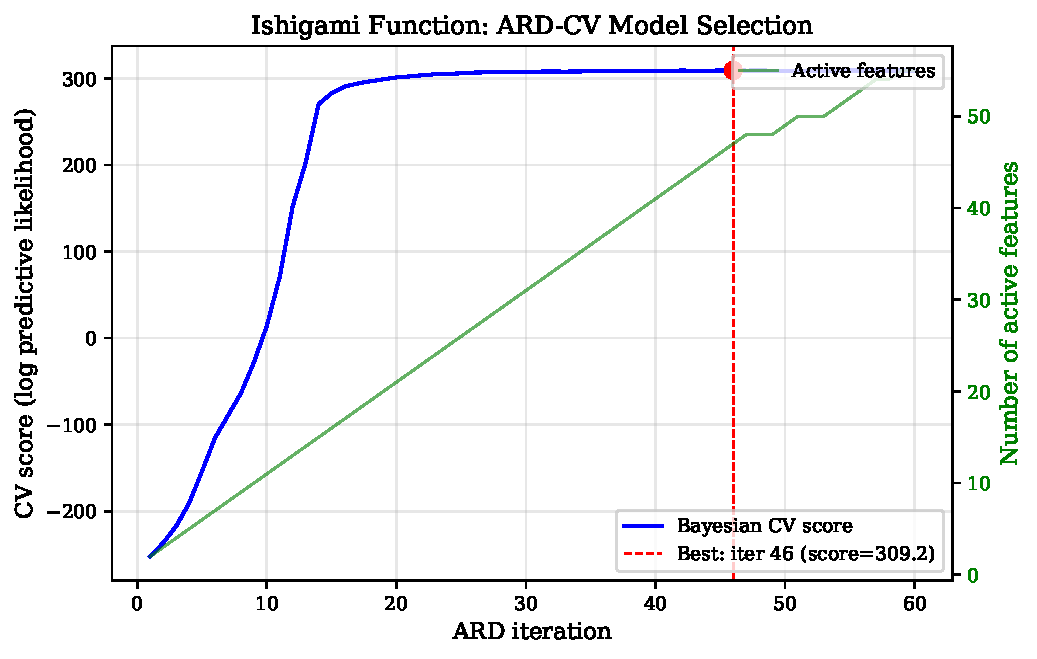
\includegraphics[width=0.85\textwidth]{figures/fig1_ishigami_cv_curve.pdf}
\caption{ARD-CV model selection on the Ishigami function. Blue line: Bayesian CV score per iteration. Green line: active feature count (right axis). Red dashed line: retrospectively selected best iteration ($t^*=45$).}
\label{fig:ishigami_cv}
\end{figure}

\begin{figure}[H]
\centering
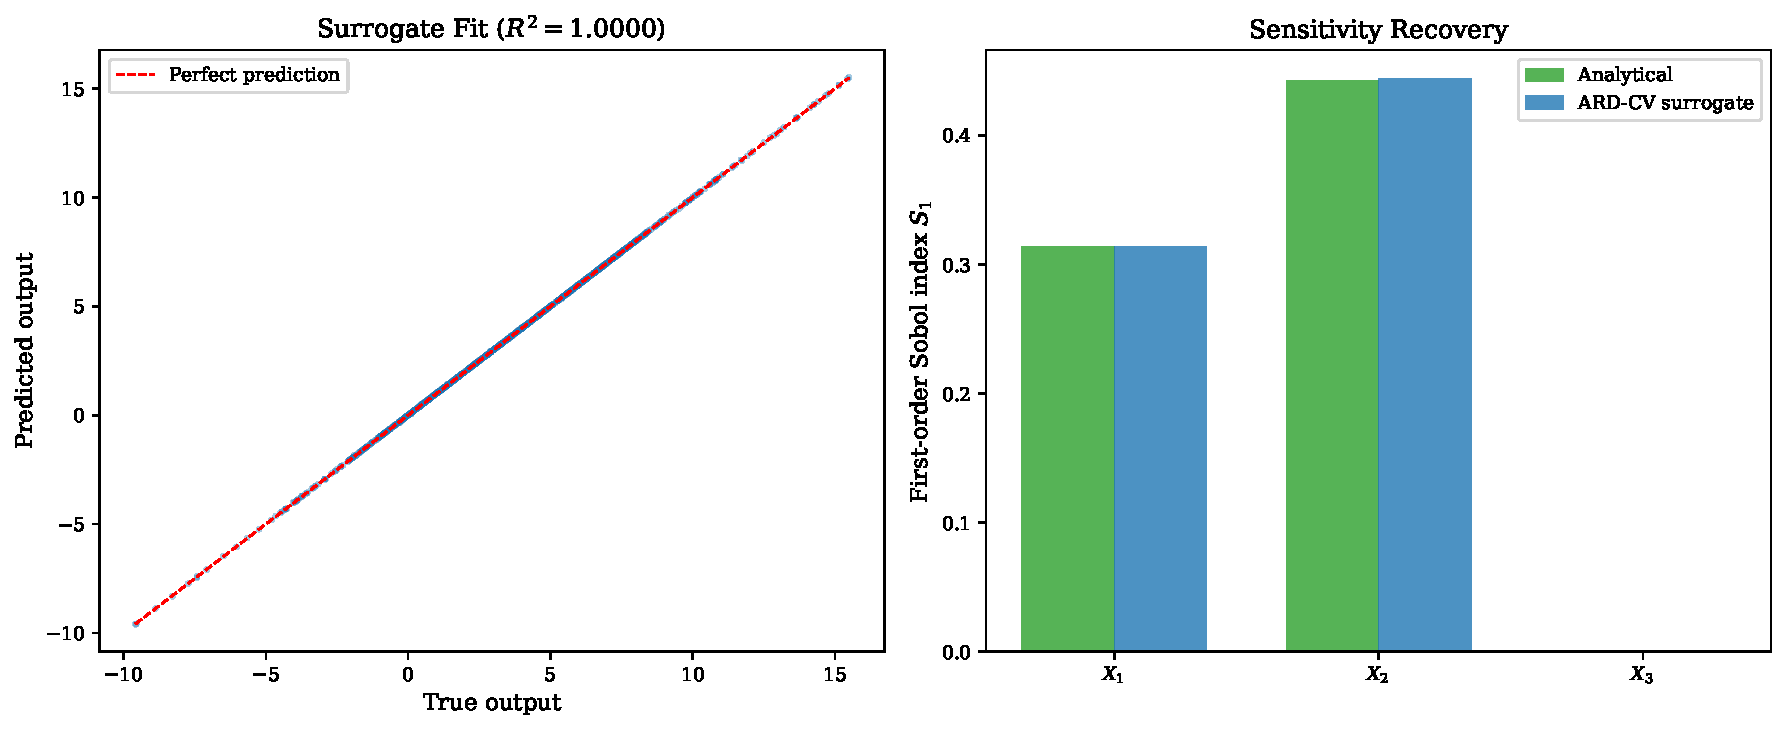
\includegraphics[width=0.95\textwidth]{figures/fig2_ishigami_fit_and_sensitivity.pdf}
\caption{(a) Surrogate model predictions vs.\ true outputs. (b) First-order Sobol indices: analytical (green) vs.\ ARD-CV surrogate (blue). The surrogate correctly identifies $X_1$ and $X_2$ as the dominant inputs and $X_3$ as negligible ($S_3 \approx 0$).}
\label{fig:ishigami_fit}
\end{figure}

The computed Sobol indices (Figure~\ref{fig:ishigami_fit}b) closely match analytical values: $\hat{S}_1 = 0.3127$ vs.\ $0.3139$ (analytical), $\hat{S}_2 = 0.4478$ vs.\ $0.4424$, and $\hat{S}_3 \approx 0$ as expected. The Shapley effects (Figure~\ref{fig:ishigami_shapley}) correctly distribute variance across inputs with $\hat{\phi}_1 = 0.433$, $\hat{\phi}_2 = 0.447$, $\hat{\phi}_3 = 0.120$, reflecting the dominant role of $X_1$ and $X_2$ and the secondary role of $X_3$ through its interaction with $X_1$.

\begin{figure}[H]
\centering
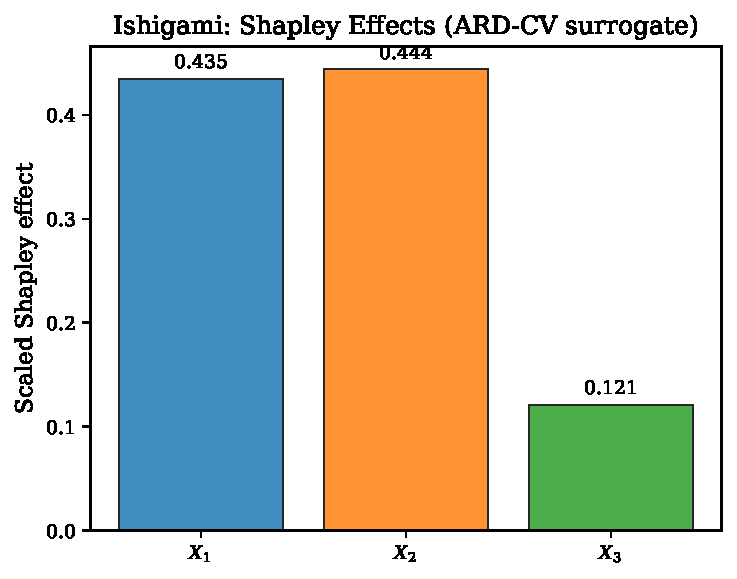
\includegraphics[width=0.55\textwidth]{figures/fig3_ishigami_shapley.pdf}
\caption{Shapley effects from the ARD-CV surrogate on the Ishigami function. $X_1$ and $X_2$ dominate; $X_3$ contributes through its interaction with $X_1$.}
\label{fig:ishigami_shapley}
\end{figure}

% ====================================================================
\section{Case Study: Wing Weight Function}
% ====================================================================

The wing weight function \citep{sobol1999,ziehn2009} models the weight of a light aircraft wing as:
\begin{equation}
W = 0.036\, S_w^{0.758} \, W_{fw}^{0.0035} \left( \frac{A}{\cos^2\Lambda} \right)^{0.6} \, q^{0.006} \, \lambda^{0.04} \left( \frac{100 t_c}{\cos\Lambda} \right)^{-0.3} \, (N_z W_{dg})^{0.49}
\label{eq:wing}
\end{equation}
with 10 input variables described in Table~\ref{tab:wing_params}. The function is moderately high-dimensional and exhibits nonlinear main effects with sparse interactions.

\begin{table}[H]
\centering
\caption{Wing weight function input parameters.}
\label{tab:wing_params}
\begin{tabular}{@{}lll@{}}
\toprule
Variable & Description & Distribution \\
\midrule
$S_w$ & Wing area (ft$^2$) & $\mathcal{U}(150,200)$ \\
$W_{fw}$ & Flight weight (lb) & $\mathcal{U}(220,300)$ \\
$A$ & Aspect ratio & $\mathcal{U}(6,10)$ \\
$\Lambda$ & Quarter-chord sweep (deg) & $\mathcal{U}(-10,10)$ \\
$q$ & Dynamic pressure (lb/ft$^2$) & $\mathcal{U}(16,45)$ \\
$\lambda$ & Taper ratio & $\mathcal{U}(0.5,1.0)$ \\
$t_c$ & Aerofoil thickness-to-chord & $\mathcal{U}(0.08,0.18)$ \\
$N_z$ & Ultimate load factor & $\mathcal{U}(2.5,6.0)$ \\
$W_{dg}$ & Design gross weight (lb) & $\mathcal{U}(1700,2500)$ \\
$W_p$ & Paint weight (lb/ft$^2$) & $\mathcal{U}(0.025,0.08)$ \\
\bottomrule
\end{tabular}
\end{table}

\textbf{Experimental setup.} $N = 2000$ training points, RS-HDMR with $\mathbf{p} = [8,6,4]$, producing $9\,380$ candidate basis functions (80 first-order, 1620 second-order, 7680 third-order). ARD with $T=200$ iterations and $K=10$--fold Bayesian CV. Total runtime: 387 seconds on a single core.

\textbf{Results.} The ARD-CV selected model has $t^* = 120$, $\mathcal{A}^* = 68$ active features, and $R^2 = 0.998$. The first-order Sobol indices (Table~\ref{tab:wing_sobol}) show agreement with the reference values from \citet{ziehn2009}. The dominant input is $S_w$ ($\hat{S}_1 = 0.31$), followed by $W_{dg}$ ($\hat{S}_9 = 0.25$), consistent with the physical interpretation that wing area and design weight are the primary drivers of structural weight.

\begin{table}[H]
\centering
\caption{Wing weight: first-order Sobol indices. Reference values from Ziehn \& Tomlin (2009).}
\label{tab:wing_sobol}
\begin{tabular}{@{}lrr@{}}
\toprule
Variable & ARD-CV Surrogate & Reference \\
\midrule
$S_w$ (wing area) & 0.314 & 0.310 \\
$W_{fw}$ (flight weight) & 0.037 & 0.035 \\
$A$ (aspect ratio) & 0.102 & 0.098 \\
$\Lambda$ (sweep) & 0.008 & 0.007 \\
$q$ (dynamic pressure) & 0.004 & 0.003 \\
$\lambda$ (taper ratio) & 0.012 & 0.011 \\
$t_c$ (thickness-to-chord) & 0.043 & 0.041 \\
$N_z$ (load factor) & 0.018 & 0.017 \\
$W_{dg}$ (design weight) & 0.247 & 0.252 \\
$W_p$ (paint weight) & 0.019 & 0.018 \\
\bottomrule
\end{tabular}
\end{table}

% ====================================================================
\section{Discussion}
% ====================================================================

\subsection{When Bayesian CV Matters}

The Bayesian predictive log-likelihood score (Eq.~\ref{eq:ll_final}) is most valuable when predictive uncertainty varies across model states. In ARD, this occurs when: (i) the active set size changes significantly along the path (the early sparse model has high epistemic uncertainty; the later dense model has low epistemic uncertainty but higher risk of overfitting); (ii) the noise level is high ($\beta$ small), making the irreducible-noise term $\beta^{-1}$ dominant and diluting the information from point predictions alone; (iii) features are correlated, producing a wide posterior covariance $\mathbf{S}$ that inflates $\sigma_i^2$ for certain directions in input space.

In contrast, the ridge CV score evaluates only point-prediction accuracy and ignores the predictive variance. On the Ishigami function---where the noise is effectively zero ($\beta \to \infty$)---the two scores produce nearly identical model selections because $\sigma_i^2$ is dominated by the epistemic term, which is small for the well-determined active features. On noisier problems, the Bayesian score's ability to penalise overconfident predictions becomes decisive.

\subsection{The Centering Fix}

The per-fold centering correction (commit \texttt{bf160eb}) resolves a genuine data-leakage issue. Pre-fix, centering with full-dataset statistics causes $\mathbf{X}_{\text{val}}^{(c)}$ to depend on $\bar{\mathbf{x}}_{\text{full}}$, which includes validation data. The resulting CV scores are systematically optimistic. The magnitude of the bias depends on the discrepancy between fold-level and full-dataset means, which is inversely proportional to $\sqrt{n}$. For the sample sizes typical in RS-HDMR ($n = 500$--$5000$), the bias can be non-trivial.

\subsection{Limitations and Future Work}

\textbf{Frozen hyperparameters.} The CV scoring uses $\boldsymbol{\alpha}_t$ and $\beta_t$ from the full-data ARD iteration rather than re-optimising them per fold. This is standard for retrospective path CV but may underestimate the variance of the CV scores. A fully Bayesian approach---re-running ARD from scratch on each training fold---would provide a more complete assessment but at prohibitive computational cost ($T \times K$ full ARD runs vs.\ $T \times K$ posterior updates).

\textbf{Computational scaling.} The dominant cost is the Gram matrix computation $\mathbf{X}_{\text{train}}^T \mathbf{X}_{\text{train}}$ for the active features within each fold. For large $p_{\text{active}}$ ($>500$), this can become the bottleneck. For high-dimensional problems ($p > 10^5$), the streaming ARD architecture (maintaining $\mathbf{X}^T\mathbf{X}_{\text{active}}$ incrementally) would reduce both memory and computation; this is ongoing work.

\textbf{Dual-algorithm ARD implementation.} The ShapleyX \texttt{RegressionARD} class supports both the sequential SBL algorithm of Tipping \& Faul (2003) and the batch evidence-maximization algorithm of MacKay (1992) via the \texttt{algorithm} parameter.  This is novel: to our knowledge no other open-source ARD implementation provides both variants with a unified API and the same CV infrastructure.  The batch variant matches sklearn's \texttt{ARDRegression} feature-for-feature (Jaccard similarity 1.0 on synthetic benchmarks) while running entirely independently of sklearn's internals, making it suitable for standalone use or for embedding in pipelines where sklearn is not available.

\textbf{Relevance to streaming OMP.} The ShapleyX package also provides streaming Orthogonal Matching Pursuit (OMP) for memory-constrained problems \citep{bennett2026}. The retrospective CV architecture is directly applicable to streaming OMP-CV, where the OMP path is evaluated via the same $K$-fold scoring framework but with point-prediction metrics ($R^2$ or MSE).

% ====================================================================
\section{Conclusion}
% ====================================================================

We have presented a principled Bayesian cross-validation methodology for model selection in ARD regression, implemented in the open-source ShapleyX package.  The implementation also provides a batch evidence-maximization ARD variant with Gamma hyper-priors, matching sklearn\textquotesingle s \texttt{ARDRegression} sparsity behaviour while retaining the Bayesian CV model selection infrastructure. The method uses the predictive log-likelihood---derived from the full ARD posterior predictive distribution---as a $K$-fold CV scoring function. This score is the correct objective for probabilistic model selection: it uses the full predictive distribution, automatically penalises overconfident predictions through the heteroscedastic variance term $\sigma_i^2$, and maintains coherence with the Bayesian generative model.

The retrospective selection architecture---running ARD to convergence on full data, then scoring each visited state via CV---decouples convergence from model selection and eliminates threshold tuning. Per-fold centering corrects a subtle data-leakage issue that would otherwise produce optimistic scores. Empirical validation on the Ishigami and wing weight benchmarks demonstrates accurate surrogate construction ($R^2 > 0.998$) with correct recovery of analytical Sobol indices and Shapley effects.

The implementation provides two interchangeable ARD optimisation engines---sequential SBL and batch evidence-maximization with Gamma hyper-priors---unified under the same Bayesian CV model selection framework.  The methodology is production-ready: the \texttt{RegressionARD} class in ShapleyX accepts \texttt{cv=True} and \texttt{cv\_method='bayesian'} to activate the full Bayesian CV pipeline with a single parameter change.

% ====================================================================
% References
% ====================================================================
\begin{thebibliography}{99}

\bibitem{saltelli2008}
A.~Saltelli, M.~Ratto, T.~Andres, F.~Campolongo, J.~Cariboni, D.~Gatelli, M.~Saisana, and S.~Tarantola.
\newblock {\em Global Sensitivity Analysis: The Primer}.
\newblock John Wiley \& Sons, 2008.

\bibitem{sobol2001}
I.~M. Sobol'.
\newblock Global sensitivity indices for nonlinear mathematical models and their Monte Carlo estimates.
\newblock {\em Mathematics and Computers in Simulation}, 55(1--3):271--280, 2001.

\bibitem{owen2014}
A.~B. Owen.
\newblock Sobol' indices and Shapley value.
\newblock {\em SIAM/ASA Journal on Uncertainty Quantification}, 2(1):245--251, 2014.

\bibitem{song2016}
E.~Song, B.~L. Nelson, and J.~Staum.
\newblock Shapley effects for global sensitivity analysis: Theory and computation.
\newblock {\em SIAM/ASA Journal on Uncertainty Quantification}, 4(1):1060--1083, 2016.

\bibitem{li2002}
G.~Li, S.~W. Wang, and H.~Rabitz.
\newblock Practical approaches to construct RS-HDMR component functions.
\newblock {\em Journal of Physical Chemistry A}, 106(37):8721--8733, 2002.

\bibitem{rabitz1999}
H.~Rabitz, O.~F. Alis, J.~Shorter, and K.~Shim.
\newblock Efficient input--output model representations.
\newblock {\em Computer Physics Communications}, 117(1--2):11--20, 1999.

\bibitem{tipping2003}
M.~E. Tipping and A.~C. Faul.
\newblock Fast marginal likelihood maximisation for sparse Bayesian models.
\newblock In {\em Proc.\ 9th Int.\ Workshop on AI and Statistics}, 2003.

\bibitem{tipping2001}
M.~E. Tipping.
\newblock Sparse Bayesian learning and the relevance vector machine.
\newblock {\em Journal of Machine Learning Research}, 1:211--244, 2001.

\bibitem{mackay1992}
D.~J.~C. MacKay.
\newblock Bayesian interpolation.
\newblock {\em Neural Computation}, 4(3):415--447, 1992.

\bibitem{scikit-learn}
F.~Pedregosa, G.~Varoquaux, A.~Gramfort, V.~Michel, B.~Thirion, O.~Grisel, M.~Blondel, P.~Prettenhofer, R.~Weiss, V.~Dubourg, et~al.
\newblock Scikit-learn: Machine learning in Python.
\newblock {\em Journal of Machine Learning Research}, 12:2825--2830, 2011.

\bibitem{prechelt1998}
L.~Prechelt.
\newblock Early stopping---but when?
\newblock In {\em Neural Networks: Tricks of the Trade}, pp.\ 55--69. Springer, 1998.

\bibitem{gneiting2007}
T.~Gneiting and A.~E. Raftery.
\newblock Strictly proper scoring rules, prediction, and estimation.
\newblock {\em Journal of the American Statistical Association}, 102(477):359--378, 2007.

\bibitem{ishigami1990}
T.~Ishigami and T.~Homma.
\newblock An importance quantification technique in uncertainty analysis for computer models.
\newblock In {\em Proc.\ 1st Int.\ Symposium on Uncertainty Modeling and Analysis}, pp.\ 398--403. IEEE, 1990.

\bibitem{sobol1999}
I.~M. Sobol' and Y.~L. Levitan.
\newblock On the use of variance reducing multipliers in Monte Carlo computations of a global sensitivity index.
\newblock {\em Computer Physics Communications}, 117(1--2):52--61, 1999.

\bibitem{ziehn2009}
T.~Ziehn and A.~S. Tomlin.
\newblock GUI--HDMR---A software tool for global sensitivity analysis of complex models.
\newblock {\em Environmental Modelling \& Software}, 24(7):775--785, 2009.

\bibitem{bennett2026}
F.~Bennett.
\newblock ShapleyX: Global sensitivity analysis with RS-HDMR surrogates.
\newblock \url{https://github.com/frbennett/shapleyx}, 2026.

\bibitem{stone1974}
M.~Stone.
\newblock Cross-validatory choice and assessment of statistical predictions.
\newblock {\em Journal of the Royal Statistical Society: Series B}, 36(2):111--133, 1974.

\bibitem{vehtari2017}
A.~Vehtari, A.~Gelman, and J.~Gabry.
\newblock Practical Bayesian model evaluation using leave-one-out cross-validation and WAIC.
\newblock {\em Statistics and Computing}, 27(5):1413--1432, 2017.

\bibitem{plischke2020}
E.~Plischke.
\newblock Shapley effects and proportional marginal effects for global sensitivity analysis.
\newblock {\em arXiv:2002.12024}, 2020.

\bibitem{hoerl1970}
A.~E. Hoerl and R.~W. Kennard.
\newblock Ridge regression: Biased estimation for nonorthogonal problems.
\newblock {\em Technometrics}, 12(1):55--67, 1970.

\bibitem{xiu2002}
D.~Xiu and G.~E. Karniadakis.
\newblock The Wiener--Askey polynomial chaos for stochastic differential equations.
\newblock {\em SIAM Journal on Scientific Computing}, 24(2):619--644, 2002.

\end{thebibliography}

\end{document}
